\documentclass{article}

%%%%%%%%%%%%%%%%%%%%%%%%%%%%%%%%
% PACKAGES
%%%%%%%%%%%%%%%%%%%%%%%%%%%%%%%%
\usepackage{times}
\usepackage{fullpage}
\usepackage{latexsym}
\usepackage{amsmath}
\usepackage{amssymb}
\usepackage{mathtools}
\usepackage{accents}
\usepackage{tikz}
\usepackage{pgfplots}
\usepackage[ruled]{algorithm}
\usepackage{algpseudocode}
\usepackage{dsfont}
\usepackage[bf]{caption}
\usepackage{hyperref}
\hypersetup{
    bookmarks=true,         % show bookmarks bar?
    unicode=false,          % non-Latin characters in AcrobatÕs bookmarks
    pdftoolbar=true,        % show AcrobatÕs toolbar?
    pdfmenubar=true,        % show AcrobatÕs menu?
    pdffitwindow=false,     % window fit to page when opened
    pdfstartview={FitH},    % fits the width of the page to the window
    pdftitle={My title},    % title
    pdfauthor={Author},     % author
    pdfsubject={Subject},   % subject of the document
    pdfcreator={Creator},   % creator of the document
    pdfproducer={Producer}, % producer of the document
    pdfkeywords={keyword1} {key2} {key3}, % list of keywords
    pdfnewwindow=true,      % links in new window
    colorlinks=true,       % false: boxed links; true: colored links
    linkcolor=red,          % color of internal links (change box color with linkbordercolor)
    citecolor=blue,        % color of links to bibliography
    filecolor=magenta,      % color of file links
    urlcolor=cyan           % color of external links
}
\usepackage{amsthm}
\usepackage{natbib}
\usepackage[capitalize]{cleveref}
\usepackage{graphicx}
\usepackage{parskip}
\usepackage{tikz} 
\usetikzlibrary{arrows,positioning} 
\pgfarrowsdeclarecombine{ring}{ring}{}{}{o}{o}
%\DeclareMathOperator{\ringarrow}{\raisebox{0.5ex}{\tikz[baseline]{\draw[ring->](0,0)--(2em,0);}}}
%%%%%%%%%%%%%%%%%%%%%%%%%%%%%%%%
% MACROS
%%%%%%%%%%%%%%%%%%%%%%%%%%%%%%%%
\newcommand{\defined}{\vcentcolon =}
\newcommand{\rdefined}{=\vcentcolon}
\newcommand{\E}[1]{\mathbb E\left[#1\right]}
\newcommand{\Var}{\operatorname{Var}}
\newcommand{\calF}{\mathcal F}
\newcommand{\sr}[1]{\stackrel{#1}}
\newcommand{\set}[1]{\left\{#1\right\}}
\newcommand{\ind}[1]{\mathds{1}\!\!\set{#1}}
\newcommand{\argmax}{\operatornamewithlimits{arg\,max}}
\newcommand{\argmin}{\operatornamewithlimits{arg\,min}}
\newcommand{\floor}[1]{\left \lfloor {#1} \right\rfloor}
\newcommand{\ceil}[1]{\left \lceil {#1} \right\rceil}
\newcommand{\eqn}[1]{\begin{align}#1\end{align}}
\newcommand{\eq}[1]{\begin{align*}#1\end{align*}}
\newcommand{\Ber}{\operatorname{Bernoulli}}
\renewcommand{\P}[1]{\operatorname{P}\left\{#1\right\}}
\newcommand{\N}[2]{\mathcal{N}\left({#1}\;,\;{#2}\right)}

\tikzset{
    %Define standard arrow tip
    >=stealth',
    %Define style for boxes
    observed/.style={
           circle,
           rounded corners,
           draw=black, thick,
           minimum width=2.5em,
           minimum height=2.5em,
           font=\footnotesize,
           text centered,
           scale=1,
           fill=blue!20!white},
     latent/.style={
           circle,
           rounded corners,
           draw=black, thick, dashed,
           minimum width=2.5em,
           minimum height=2.5em,
           font=\footnotesize,
           text centered,
           fill=black!10!white
           },
     empty/.style={
           circle,
           rounded corners,
           minimum width=.5em,
           minimum height=.5em,
           font=\footnotesize,
           text centered,
           },
    % Define arrow style
    pil/.style={
           o->,
           thick,
           shorten <=2pt,
           shorten >=2pt,},
    sh/.style={ shade, shading=axis, left color=red, right color=green,
    shading angle=45 }  
}


%%%%%%%%%%%%%%%%%%%%%%%%%%%%%%%%
% THEOREMS
%%%%%%%%%%%%%%%%%%%%%%%%%%%%%%%%
\theoremstyle{plain}
\newtheorem{theorem}{Theorem}
\newtheorem{proposition}[theorem]{Proposition}
\newtheorem{lemma}[theorem]{Lemma}
\newtheorem{corollary}[theorem]{Corollary}
\theoremstyle{definition}
\newtheorem{definition}[theorem]{Definition}
\newtheorem{assumption}[theorem]{Assumption}
\newtheorem{remark}[theorem]{Remark}
\newtheorem{example}[theorem]{Example}

\title{Partial Identifiability}


\begin{document}
\def\ci{\perp\!\!\!\perp}

\subsection*{Adjustment}

\begin{figure}[H]
	\centering    
          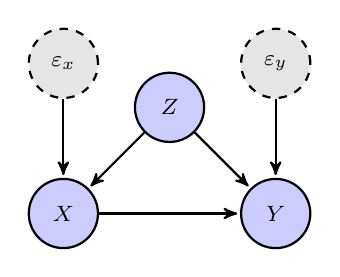
\begin{tikzpicture}[->,>=stealth',shorten >=1pt,auto,node distance=1cm,
  thick,main node/.style={observed}, hidden/.style={empty},background rectangle/.style={fill=olive!45}]
 %nodes
\node[main node](2){$X$};
\node[main node, above right=of 2](3){$Z$};
\node[main node, below right=of 3](4){$Y$};
\node[latent, above=of 2](5){$\varepsilon_x$};
\node[latent, above=of 4](6){$\varepsilon_y$};
 \path[every node/.style={font=\tiny}]
    (3) edge (2) edge (4)
    (2) edge (4)
    (5) edge (2)
    (6) edge (4);
\end{tikzpicture}
\end{figure}

To estimate the causal effect of $X$ on $Y$, we need to condition on $Z$ so as to block the backdoor path $X \leftarrow Z \rightarrow Y$. 

\eq {
P(Y|do(X=x)) = \sum_{z \in \mathcal{Z}}P(Y|X=x,Z=z)P(Z)
}

With a binary treatment $X$ we can also write:

\eq{
ATE = E(Y|do(X=1)) - E(Y|do(X=0))
}

This assmumes $Z$ is fully observable, ie there are no unobservable variables, $U$ that cause both $X$ and $Y$. 

\subsection*{Covariate Shift}

Seperate from the problem of adjustment, lets define covariate shift.

\begin{itemize}
\item We have training data $d_{train} = \set{(x_1,y_1),...,(x_n,y_n)}$ sampled from $P(X,Y) = P(X)P(Y|X)$.
\item The test data $d_{test} = \set{(x'_1,y'_1),...,(x'_{n'},y'_{n'})}$ is assumed to be sampled from $Q(X)P(Y|X)$, where $Q(X) \neq P(X)$. As usual for test data, we observe only the inputs $\set{x'_1,...,x'_{n'}}$
\item We wish to use the training data to learn a hypothosis/function $h:\mathcal{X} \rightarrow \mathcal{Y}$ that minimises $\sum_{i = 1}^{n'}\mathcal{L}(h(x'_i,y'_i))$, where $\mathcal{L}$ is some loss.
\end{itemize}

The covariate shift assumption is that $P(Y|X)$ has not changed. 

%This assumption is plausible if $X$ causes $Y$ and we imagine a mechanism that maps $\mathcal{X}$ to $\mathcal{Y}$ that is independent of the input distribution. If $Y$ causes $X$ then we would expect that $P(X)$ and $P(Y|X)$ would in general be related, such that a shift in $P(X)$ would lead us to ancipate that $P(Y|X)$ might also have changed.

Although we have assumed the underlying mapping, $P(Y|X)$, we are trying to learn has not changed between the test and the train data we still need to adapt standard prediction algorithms as otherwise (through a preference for 'simple' functions) we may select a function that fits well where $P(X)$ is high but performs badly where $Q(X)$ is high. There are some situations that require no adaptation. For example, if the true function is linear and we fit an (unregularized) linear model, then model that is in expectation optimal on the training data is also optimal for the test data. Another interesting example is if the model is a Gaussian process \cite{}. 

\subsection*{Covariate shift in the adjustment problem}

In the adjustment problem, we have observational training data, $d_{train} = \set{(x_1,z_1,y_1),...(x_n,z_n,y_n)} \sim P(Z,X)P(Y|Z,X)$. If we intervene and set $X=x$ then the data will be sampled from $P(Z)\delta(X-x)P(Y|Z,X)$. Note that the covariate shift assumption is satisfied in this scenario, $P(Y|Z,X)$ does not change between the train and test settings. What has changed is the joint distribtion $P(X,Z)$.







\end{document}

